\documentclass[logo,reportComp]{thesis}
\usepackage[cpp,pseudo]{mypackage}

\title{高级编程技术实验报告}
\subtitle{实验二:最短路径}
\school{数据科学与计算机学院}
\author{陈鸿峥}
\classname{17大数据与人工智能}
\stunum{17341015}
\headercontext{高级编程技术实验报告}
% \authorremark{本实验报告用\LaTeX撰写,创建时间:\builddate\today}
\lstset{language=python}

\begin{document}

\maketitle

\section{问题描述及求解思路}
\subsection{创建数据结构}
对于\verb'WeightedEdge'的初始化如下
\begin{itemize}
    \item \verb'__init__':调用父类构造函数\verb'Edge.__init__'进行初始化
    \item \verb'get_total_distance'和\verb'get_outdoor_distance':均直接返回值
    \item \verb'__str__':类似\verb'Edge'类的字符转化方法
\end{itemize}

对于\verb'Digraph'的初始化如下
\begin{itemize}
    \item \verb'add_node':先用\verb'has_node'判断结点是否在结点集合中,如果不存在则报错\verb'raise ValueError';否则添加结点到集合中
    \item \verb'add_edge':同样先判断结点是否在结点集合中,如果存在则判断是否新加结点,如果是新加结点则创建一个新列表,否则直接插入原有列表中
\end{itemize}

\subsection{创建校园地图}
下面问题的答案在\verb'ps2.py'中也可以找到
\begin{itemize}
    \item [a.] 每一个图结点代表校园里的一栋大楼,每一条边代表一栋大楼和另一栋大楼相邻(有路可走),距离/边权则代表一栋大楼到另一栋大楼的距离。
    \item [b.] \verb'load_map':先创建一个空对象\verb'g=Digraph()',利用\verb'with open(map_filename,"r") as file'打开文件,防止文件不存在仍继续执行。
    然后遍历文件的每一行,通过\verb'split'函数按照空格分割,同时可以如下用四元组直接赋值。
\begin{lstlisting}
(src,dst,tot_dist,outdoor_dist) = line.split(' ')
\end{lstlisting}
    判断图\verb'g'中是否存在源结点和汇结点,如果不存在则添加。
    然后创建有权边\verb'WeightedEdge',通过\verb'add_edge'添加入图\verb'g'中。
    \item [c.] 如下测试输出是否合规。
\begin{lstlisting}
school_map = load_map("test_load_map.txt")
print(school_map)
\end{lstlisting}
\end{itemize}

\subsection{用优化DFS寻找最短路径}
\subsubsection{目标函数}
\begin{itemize}
\item 目标函数:最小化从源结点到汇结点的距离
\item 限制条件:出校外的距离不能超过\verb'max_dist_outdoors'
\end{itemize}

\subsubsection{实施最优路径}
伪代码已经在题目描述中给出,下面是完整代码,原题注释已删除。
\begin{lstlisting}
def get_best_path(digraph, start, end, path, max_dist_outdoors, best_dist,
                  best_path):
    # not valid nodes
    if not (digraph.has_node(Node(start)) and digraph.has_node(Node(end))):
        raise ValueError
    # recursion termination
    elif start == end:
        if path[1] < best_dist:
            best_path = copy.deepcopy(path[0])
            best_dist = path[1]
    # get deeper
    else:
        for edge in digraph.get_edges_for_node(Node(start)):
            dst = edge.get_destination()
            if dst in path[0]: # avoid cycles
                continue
            tmp_path = copy.deepcopy(path)
            tmp_path[0].append(dst)
            tmp_path[1] += edge.get_total_distance()
            tmp_path[2] += edge.get_outdoor_distance()
            if tmp_path[2] > max_dist_outdoors: # not satisfy the constraint
                continue
            if tmp_path[1] > best_dist: # cut!!! greatly reduce time
                continue
            (tmp_best_path,tmp_best_dist) = get_best_path(digraph,dst,end,
                tmp_path,max_dist_outdoors,best_dist,best_path)
            if tmp_best_dist < best_dist: # update best path
                best_path = tmp_best_path
                best_dist = tmp_best_dist
    return (best_path,best_dist)
\end{lstlisting}

这里有几个点需要注意:
\begin{itemize}
    \item 每次对\verb'path'进行修改之前都记得要进行\textbf{深拷贝},仅仅是数组的\verb'.copy'是不够的,因为\verb'path'是一个嵌套列表。
    故这里我采用了\verb'copy.deepcopy'的方式进行深拷贝
    \item 为了避免成环的情况的情况,先判断新结点是否已经在路径上,如果是则直接跳过
    \item 对于新加入的边,如果总长度已经超过最优长度,则后面的搜索都可以被裁剪掉,这将大大缩短运行时间(见图\ref{fig:no_cut}和图\ref{fig:cut}的比较)
    \item 每次迭代完返回都要将值赋给临时变量\verb'tmp_best_path'和\verb'tmp_best_dist',在当前层所有结点都遍历完后才返回最优路径
\end{itemize}

\subsubsection{实施有向DFS}
这里直接调用上一问的\verb'get_best_path'函数即可。代码如下,原题注释已删除。
\begin{lstlisting}
def directed_dfs(digraph, start, end, max_total_dist, max_dist_outdoors):
    (best_path,best_dist) = get_best_path(digraph,start,end,[[start],0,0],max_dist_outdoors,max_total_dist,[])
    if best_path == []:
        raise ValueError
    else:
        return best_path
\end{lstlisting}

注意\verb'start'要先存入初始列表中,然后将最优路径长度设为最大路径长。
如果没有比最大路径长更小的路径,则对应的\verb'best_path'也会为空,进而报错\verb'raise ValueError'。

\section{代码}
代码实施及注释请见附件\verb'graph.py'、\verb'ps2.py'。
自己写的测试样例见\verb'test_load_map.txt'。

\section{运行截图}
实验运行结果如下面几幅图片所示。
\begin{figure}[H]
\centering
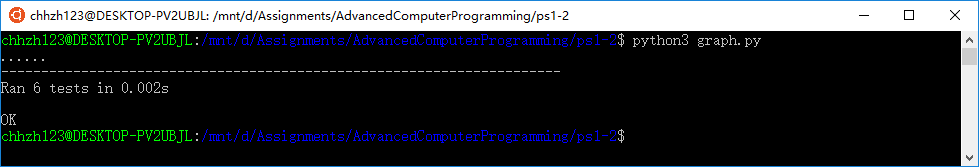
\includegraphics[width=\linewidth]{fig/graph.PNG}
\caption{问题1结果,测试样例全通过}
\label{fig:graph}
\end{figure}

\begin{figure}[H]
\centering
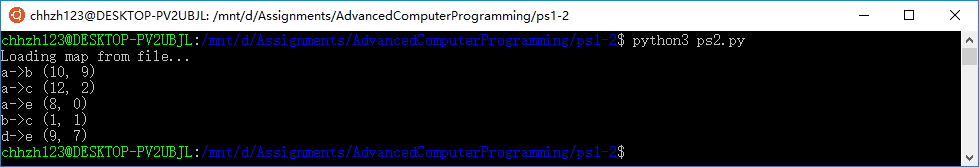
\includegraphics[width=\linewidth]{fig/test.PNG}
\caption{问题2结果,测试样例输出正常}
\label{fig:test}
\end{figure}

\begin{figure}[H]
\centering
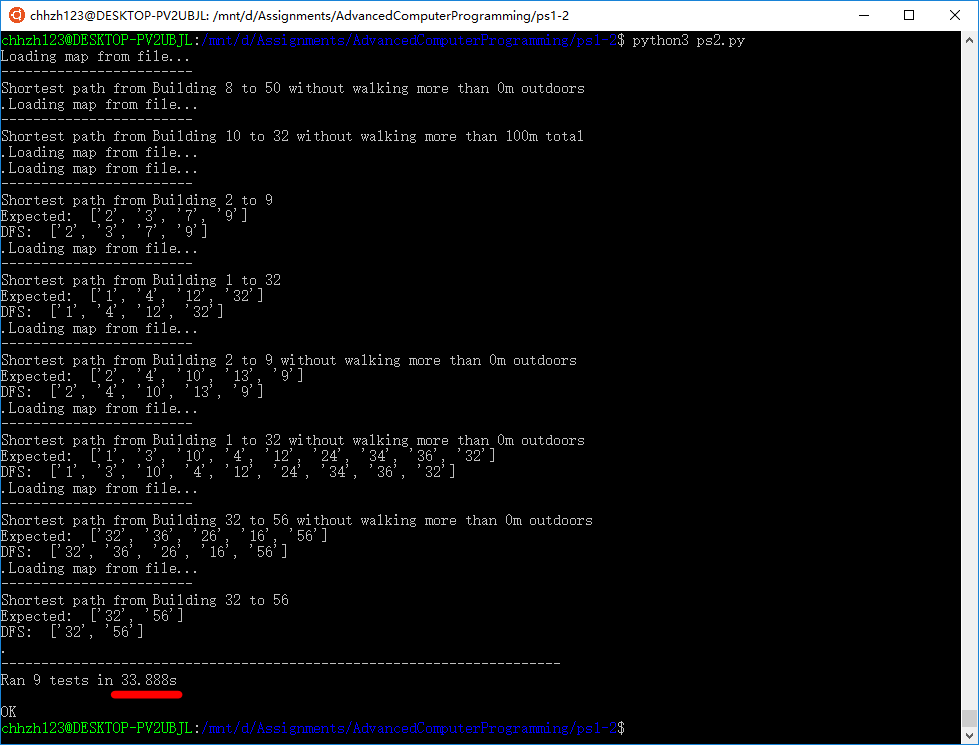
\includegraphics[width=\linewidth]{fig/no_cut.PNG}
\caption{问题3结果,测试样例全通过。没有剪枝,相当于枚举所有情况,速度非常慢}
\label{fig:no_cut}
\end{figure}

\begin{figure}[H]
\centering
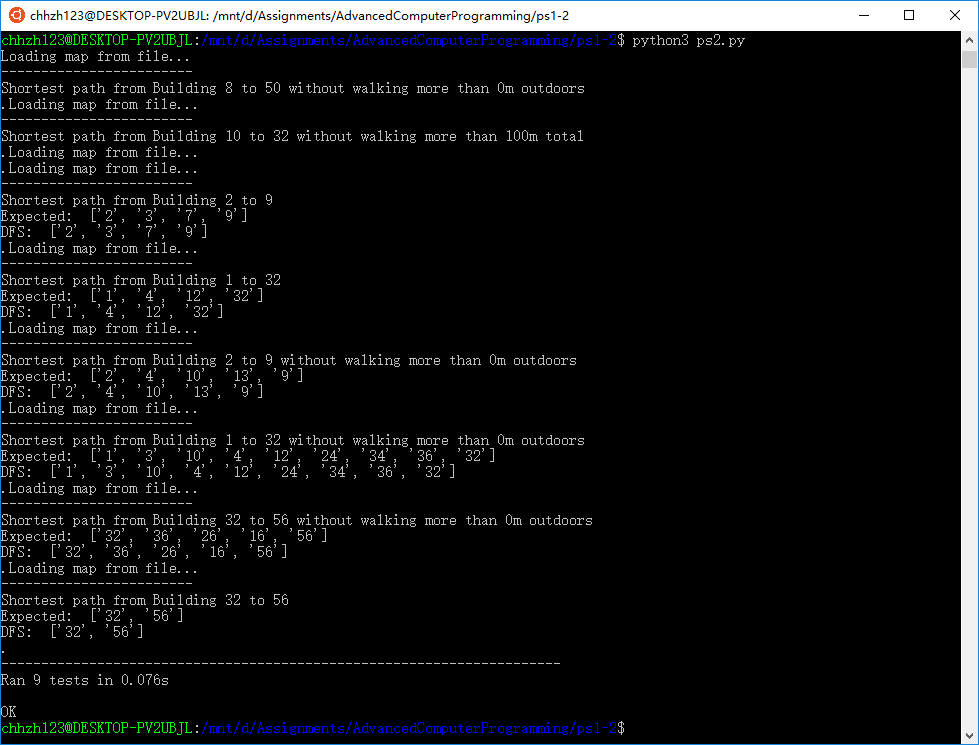
\includegraphics[width=\linewidth]{fig/cut.PNG}
\caption{问题3结果,测试样例全通过。运用剪枝,速度大幅提升}
\label{fig:cut}
\end{figure}

\end{document}

% 实验提交内容
% 邮件主题,作业文件命名规范(学号、姓名)
% 文档pdf格式(问题、求解思路、代码、注释、运行截图)
% 考虑健壮性、可读性
% 极端样例